\chapter{敏捷开发和Scrum}
\label{敏捷开发和scrum}

敏捷软件开发越来越流行了,而且基本深入人心。技术水平高的人尤其推崇。

当我们学习编程时,本性都是敏捷的,谁都不想浪费时间。只是进入企业(不管大小)后,由于管理的需要,产生了不必要的浪费,也就显得不太敏捷了。

瀑布V模型在早期开发周期长,需求变化少的情况下还是很不错的,只是互联网时代软件开发技术日新月异,更新越来越快,这又不得不回到原来的思想,精简管理来降低浪费。

由此不要抱怨敏捷,它只是揭开了软件开发的遮羞布而已。

敏捷是由很多技术实践结合在一起的,依靠有经验的开发者去实施。

\section{工作环境}
\label{工作环境}

不需要电脑,积极回答问题,并多多提问。

\section{简单历史}
\label{简单历史}

敏捷这个术语早期有人叫轻量级(lightweight)软件过程,来区别于CMM、RUP等重量级软件过程。后来又觉得本质不是轻重的问题,所以又改成敏捷(Agile)。

\begin{figure}[htbp]
\centering
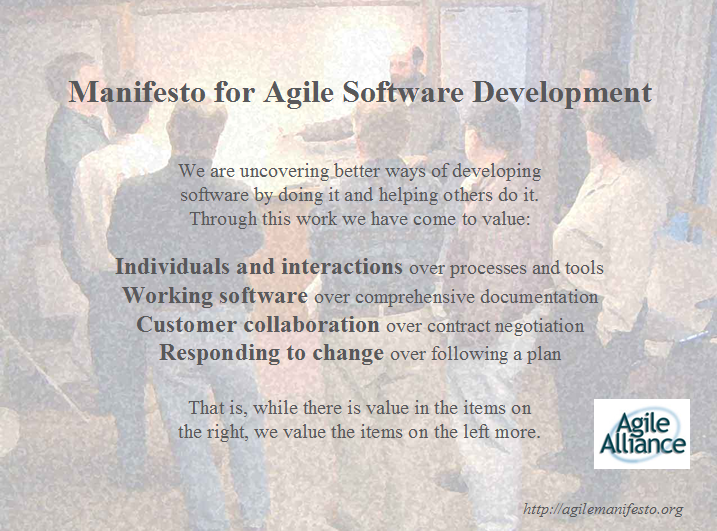
\includegraphics[keepaspectratio,width=\textwidth,height=0.75\textheight]{img/18333fig0101-tn.png}
\caption{敏捷宣言}
\end{figure}

敏捷的技术实践在敏捷出现前就出现了,如持续集成,代码共享,结对编程。甚至是那些敏捷流派,如XP、Scrum、FDD都早就有了。只是这些技术先驱们觉得单打独斗太累,因此在一次聚会中一起创建了敏捷宣言\footnote{http:/\slash agilemanifesto.org\slash iso\slash zhchs\slash }。

\subsection{敏捷流派}
\label{敏捷流派}

从2004年起,敏捷开始展露锋芒,主要原因是恰好互联网企业需要快速开发,快速交付。他们就顺理成章地采用了敏捷的方式。

同时传统企业开始感受到了压力,碰到了问题,需要改进了,看看别人都敏捷了,开始跟风(褒义)了,这就碰到了选择的问题。记住,只有等你到了一定的水准后,才能无招胜有招。早期还是要学些固定套路的,这些套路就是不同的敏捷开发过程。

\begin{itemize}
\item XP(极限编程)较早出现在中国的原因,得益于当初翻译的几本书(2001年),不过有点极端了,很多传统企业都不能适应。

\item Scrum是一个框架,概念清晰,比较容易上手(狡猾),当然它还是得和其他实践同步开展。不管怎么样,Scrum越来越流行了;当然骂声也不少,认为它什么都没讲,太虚了。实际上他们大多数人把自身的问题归结于Scrum了。

\item FDD(Feature Driven Development)等还有一些其他的过程,声音慢慢就越来越少了。猜想商业是一方面,推动者的能力或兴趣也是一方面。

\end{itemize}

这里,我们主要以Scrum来讲解敏捷,但千万别以为Scrum就是敏捷。可以阅读相关知识来了解更多的敏捷。

\section{Scrum 基本知识}
\label{scrum基本知识}

Scrum\footnote{http:/\slash zh.wikipedia.org\slash wiki\slash Scrum}是迭代式增量软件开发过程,也是一种敏捷软件开发的框架,通常用于敏捷软件开发。Scrum在英语的意思是橄榄球里的争球。

\subsection{基本角色}
\label{基本角色}

Scrum是一个包括了一系列实践和预定义角色的过程框架。Scrum中的主要角色包括:

\begin{enumerate}
\item \textbf{Scrum Master}是来确保团队合理的运作Scrum,并帮助团队移除实施中的障碍。

\item \textbf{产品负责人(PO: Product Owner)},确定产品的方向和愿景,定义产品发布的内容、优先级及交付时间,为产品负责。

\item \textbf{开发团队(Team)},一个跨职能的小团队,人数5--9人,团队拥有交付可用软件需要的各种技能。

\end{enumerate}

\begin{figure}[htbp]
\centering
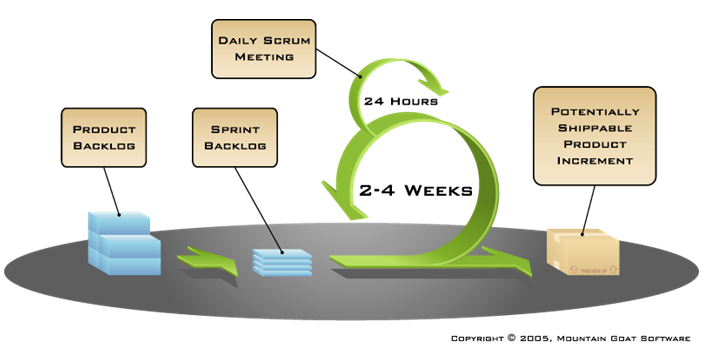
\includegraphics[keepaspectratio,width=\textwidth,height=0.75\textheight]{img/18333fig0102-tn.png}
\caption{Scrum框架}
\end{figure}

\subsection{框架过程}
\label{框架过程}

在每一个Sprint(两到四周的周期,其长度由开发团队决定)当中,开发团队创建可用的(可以随时推出)软件的一个增量。每一个Sprint所要实现的功能来自\textbf{产品待办事项列表(Product backlog)}。

产品待办事项列表是按照优先级排列的要完成的工作的概要需求,在团队的\textbf{计划会议(Planning meeting)}中,PO给出各个功能的优先级,开发团队一起决定在下一次Sprint中他们能够承诺完成多少功能,这就形成了\textbf{Sprint待办事项列表(Sprint backlog)}。

在Sprint过程中,没有人能够变更Sprint待办事项列表,这意味着在Sprint中需求是被冻结的(No Change)。

\textbf{每日站立会议(Daily standup meeting)}一般定在早上,持续10分钟左右,每个团队成员需要回答三个问题来了解整个的运行情况和潜在的风险:

\begin{enumerate}
\item 昨天你完成了哪些工作?

\item 今天你打算做什么?

\item 完成你的目标是否存在什么障碍?

\end{enumerate}

在Sprint结束时,会有一个\textbf{评审会议(Review meeting)}来检查一下功能是否按照产品负责人要求地完成了,质量应该是由团队保证的,而不是产品负责人或其他人负责。

评审会议后的\textbf{回顾会议(Retrospective meeting)}是团队自己帮助自己发现问题,并提出行之有效的方式进行提高,所以这不是由其他人来组织的。

\subsection{常用的实践}
\label{常用的实践}

管理Scrum过程有很多实施方法,如即时贴(yellow stick)、燃尽图(burndown chart )、白板(whiteboard)。Scrum最大的好处之一是它非常容易学习,而且启动Scrum应用并不需要太多的投入。

\begin{figure}[htbp]
\centering
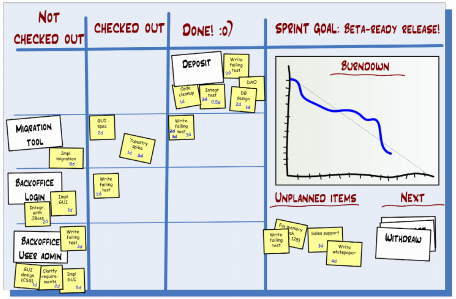
\includegraphics[keepaspectratio,width=\textwidth,height=0.75\textheight]{img/18333fig0103-tn.png}
\caption{每日例会中的任务白板(图来自《硝烟中的Scrum和XP》一书)}
\end{figure}

\section{相关知识}
\label{相关知识}

敏捷这个范畴很大,在过程这个方面,建议看看XP和Lean、看板等内容。

\section{课后练习}
\label{课后练习}

学会使用白板来做团队任务的分配,并且开始体会团队合作和企业中的工作任务和以前的不同。

\begin{enumerate}
\item 在Wiki系统中,各自创建自己的个人主页。

\item 敏捷团队到底要不要团队组长(Team leader),简单阐述想法,记录在Wiki中。

\item 一个敏捷团队几个人是最适合的,简单阐述想法,记录在Wiki中。

\item Scrum周期多长是最合适的,简单阐述想法,记录在Wiki中。

\end{enumerate}

\section{小结}
\label{小结}

敏捷听起来很虚,但是实际上回归了软件开发的本质,关注需求,团队合作,不断进步。

\section{参考阅读}
\label{参考阅读}

\begin{enumerate}
\item 硝烟中的Scrum和XP: http:/\slash www.infoq.com\slash cn\slash minibooks\slash scrum-xp-from-the-trenches

\item 看板和Scrum——相得益彰:http:/\slash www.infoq.com\slash cn\slash minibooks\slash kanban-scrum-minibook-cn

\item 你的Scrum检查列表:http:/\slash www.infoq.com\slash cn\slash minibooks\slash scrum-checklists-cn

\item What is scrum? http:/\slash www.scrumalliance.org\slash pages\slash what\_is\_scrum

\end{enumerate}

\chapter{版本控制Git和代码审阅Gerrit}
\label{版本控制git和代码审阅gerrit}

如果你还停留在SVN阶段,或者从没有玩过Git,那太落伍了。Git是版本控制的一个飞跃,它极大的提高了软件开发的效率。

代码审阅有好几种方式,走读式效果不佳(有点事后诸葛亮的味道),结对编程(Pair Programming)一直是蛮多人推荐的方式,但真正在企业中实施成功的不是很多,不过还是值得推荐的。

基于Gerrit方式的代码审阅有很多的优点,能很好得满足企业的需要。

\section{工作环境}
\label{工作环境}

\begin{itemize}
\item 服务器端推荐用 Gerrit \href{http://code.google.com/p/gerrit/}{http:/\slash code.google.com\slash p\slash gerrit\slash }

\item 客户端用Windows版的Git:\href{http://code.google.com/p/msysgit/}{http:/\slash code.google.com\slash p\slash msysgit\slash }

\end{itemize}

\section{什么是Git}
\label{什么是git}

Git最早是Linus用于Linux内核开发的版本控制工具。与常用的版本控制工具 CVS、Subversion 等不同, 它采用了分布式版本库的方式,不需服务器端软件支持,使源代码的发布和交流极其方便。 

Git的速度很快,既然它能应付Linux kernel这样的大项目,那么相信对大多数的企业软件的协作开发和代码量,它也是能胜任的。

Git最为出色的是它的合并跟踪(Merge tracing)能力和强大的社区支持。

\subsection{集中式和分布式}
\label{集中式和分布式}

企业常用的SVN和ClearCase是集中式版本控制系统,服务器架在IT环境中,本地只是签出代码的一个快照。很多操作如历史记录查询都必须要连接到服务器才行。只要依赖网络,就会带来不必要的麻烦,比如在家办公。

分布式顾名思议就是代码仓库是可以分布在各处的,那样你就可以做很多以前必须要配置管理员参与的事情,如分支。当然它也带来一定的复杂性,早期可能还不太适应。有兴趣的朋友可以在附录B看看我的一些推广经验:“
企业版本控制的改革:走向Git”。

\begin{figure}[htbp]
\centering
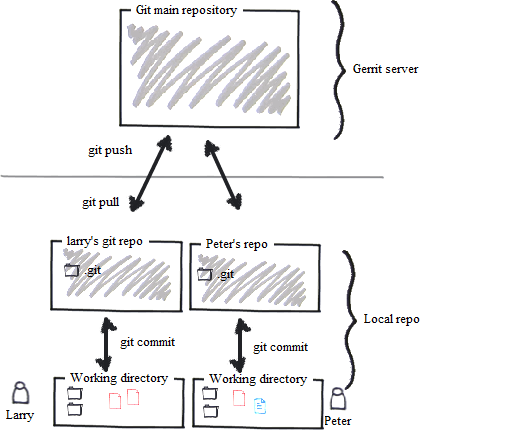
\includegraphics[keepaspectratio,width=\textwidth,height=0.75\textheight]{img/18333fig0201-tn.png}
\caption{Git分布式版本控制}
\end{figure}

\section{Git基本用法}
\label{git基本用法}

Git的学习曲线相对来说还是有点陡的,但只要掌握了基本的一些命令,开始日常的工作就没有问题了。

\subsection{安装}
\label{安装}

先装好Windows版的Git(\href{http://code.google.com/p/msysgit/downloads/list?can=3&q=official+Git}{``Git for windows''}\footnote{\href{http://code.google.com/p/msysgit/downloads/list?can=3\&q=official+Git}{http:/\slash code.google.com\slash p\slash msysgit\slash downloads\slash list?can=3\&q=official+Git}}),很多人老是说装msysgit,实际上我们要的只是Git的工作环境,而msysgit是一个含有整套源码环境的系统(如C编译器)完整包,除非你是个Git极客,否者别自寻麻烦。

缺省安装就可以了,除非你是专家,否则别选Putty(一种常用的远端控制台软件)的SSH。初学者80\%的Git的问题出在SSH连接上。

\subsection{配置 Git}
\label{配置git}

首先要告诉Git你是谁,怎么联系你,这样在代码库中才能找到提交者;同时界面也可设置成彩色来方便阅读。在SHELL环境下进行如下全局配置:

\begin{lstlisting}[language=bash]
$ git config --global user.name "Your name"  
$ git config --global user.email "Your email address"
$ git config --global color.ui auto
\end{lstlisting}

\texttt{--global}就是把全局配置放在你的HOME下 \texttt{\ensuremath{\sim}\slash .gitconfig},下面两条命令都可看到全局定义。

\begin{verbatim}
$ less ~/.gitconfig 
$ git config -l --global
\end{verbatim}

\subsection{建立本地 Git 仓库}
\label{建立本地git仓库}

既然是分布式,就可以直接在本地创建Git仓库了。先生成一个干净目录\texttt{helloworld}并初始化成Git仓库。

\begin{lstlisting}[language=bash]
$ cd ~
$ mkdir helloworld
$ cd helloworld
$ git init   # 初始化本地仓库
Initialized empty Git repository in c:/Users/larrycai/helloworld/.git/
\end{lstlisting}

养成习惯经常看看目录下有什么变化了。

\begin{lstlisting}[language=bash]
$ find .
.
./.git
./.git/config
./.git/hooks
...
./.git/hooks/update.sample
./.git/info
./.git/objects
./.git/refs
./.git/refs/heads
./.git/refs/tags
\end{lstlisting}

你会发现新建了\texttt{.git}目录,在下面还有很多东西,自己瞅瞅,琢磨琢磨,这也是平时自我提高的一个办法。不管怎样,这就是你的本地Git仓库了。

\subsection{第一个提交}
\label{第一个提交}

然后可以试着加入一些代码并签入本地版本库。

\begin{lstlisting}[language=bash]
$ cat "Hello Git World" > README # 建一个空文件
$ git status # 会发现报告红色的未跟踪的文件
$ touch README # 创建空文件
$ git add README # 加入暂存(stage)区
$ git status & find . # 变绿色,跟踪了。产生一个索引
$ git commit -am "add first empty file" # 签入代码到本地,要养成好习惯写好提交的注释。
$ git status & find . # 干净了,索引变化了。
$ git log
$ git blame # 查看谁改的
\end{lstlisting}

要细心体会每次的变化,就这么简单,也不那么容易。

\subsection{Git分支(Branch)和合并(Merge)}
\label{git分支(branch)和合并(merge)}

为了不影响团队其他成员的开发,常常建立一个分支(Branch)用来开发新功能和修改bug,等开发完成后,再合并(merge)到主分支(master)上供其他人使用。

分支和合并在其他大多数的版本控制系统中(如SVN,ClearCase)都是高级课程,而在Git中,一会儿就学到了。记住,在分布式版本控制系统中,这是一种很常用的工作方式。

一个Git仓库可以维护很多开发分支并\texttt{快速}切换,这是推荐的工作方式,而在SVN中,分支是尽量避免的。

\begin{verbatim}
$ git branch bug123 #创建关于 bug 123的分支
$ git branch  # 看看有哪些分支,master是主分支。
  bug123
* master
$ git checkout bug123 # 切换到bug123分支。
Switched to branch 'bug123'
$ git checkout -b feature234 # 创建并直接切换到feature234分支
\end{verbatim}

当需要合并时,切换到需要合并的分支上,如果需要,可以使用kdiff等软件。

\begin{verbatim}
$ git checkout master # 切换到主分支
$ git merge bug123 # bug123已解决,合并bug123
$ git branch -d bug123 # bug123没用了,可以删除这个分支了。
\end{verbatim}

\subsection{Git变基(Rebase)}
\label{git变基(rebase)}

在两个分支之间同步的操作除了合并,还有一个类似的命令叫变基(rebase)。它就是把你的分支重新更新到新的基础之上。

\begin{verbatim}
$ git checkout master 
$ git checkout -b bug123 # 从主分支工作在bug123分支上
$ git rebase master # 变基到最新的主分支的内容,继续修改bug123
\end{verbatim}

\subsection{Git标记(Tag)}
\label{git标记(tag)}

一般在发布前,我们需要打一个标记(Tag),表明这是一个重要的点,以后可以很方便地把当前的状态恢复,省得记录某个固定的签入了。

\begin{verbatim}
$ git tag -a v1.0.0 -m "official release for version 1.0.0" # 创建里程碑并加注释
$ git tag # 列出所有的里程碑
$ git checkout v1.0.0 # 以后可以很方便地签出里程碑 v1.0.0
\end{verbatim}

\section{Git远程仓库连接}
\label{git远程仓库连接}

到现在为止,我们一直在本地练习,该把代码上传到Git服务器了。Git服务器有好几种,如Gitolite、Gerrit。企业建议用Gerrit。

Gerrit是基于SSH协议用Java实现的Git服务器,谷歌Android开源项目就是使用Gerrit。

\subsection{在Gerrit中注册}
\label{在gerrit中注册}

使用前,需要在Gerrit中注册,首先用正确的账号和密码登陆,然后上传你的SSH公钥。

SSH公钥是要用\texttt{ssh}命令产生的。运行\texttt{ssh-keygen}就会在根目录下创建\texttt{.ssh}目录和生成公私密钥文件\texttt{id\_rsa.pub},\texttt{id\_rsa}。

\begin{verbatim}
$ ssh-keygen # 提示输入密码时回车用空密码就可以了!
\end{verbatim}

\texttt{id\_rsa.pub}就是公钥文件,上传并放在你的Gerrit账户下面。以后Git的相关命令就通过SSH来验证。

\subsection{Git克隆(Clone)}
\label{git克隆(clone)}

从远端Git服务器上把代码从远端Git仓库拿到本地的操作就叫克隆(Clone)。

\begin{verbatim}
$ git clone ssh://larrycai@gerritserver.company.com:29418/gameoflife.git
\end{verbatim}

如果一切正确,代码和它的全部历史就到了本地,记住你拿到的是完整的Git仓库,只是在本地而已,否则就不是分布式了。可以看看\texttt{.git}目录,或者打一下\texttt{git log}体会一下。

上面的命令中:

\begin{itemize}
\item \texttt{ssh:/\slash } 代表了访问的协议,后面的\texttt{29418}是SSH协议的通信端口,Gerrit不使用缺省端口\texttt{22}。

\item \texttt{larrycai} 是Gerrit中的账号ID,如果和你本地的ID相同可以省略。

\item \texttt{gerritserver.company.com} 是你企业使用用Gerrit的Git服务器。

\item \texttt{gameoflife.git} 是Git仓库名字,一般习惯以\texttt{.git}作为后缀。

\end{itemize}

\subsection{Git推送\slash 拉(Push\slash Pull)}
\label{git推送拉pushpull}

克隆后,你就可以在本地创建分支修改代码,并使用前面学习的Git命令来进行版本控制。

当完成一定的任务,代码修改完毕后,就可以考虑推送(Push)到远程仓库和别人共享。

\begin{verbatim}
$ git push 
\end{verbatim}

命令格式是: \texttt{git push [remote-name] [branch-name]},缺省是\texttt{origin}和\texttt{master}。克隆操作会自动使用默认的master和 origin名字。可以看看\texttt{.git\slash config}文件。

同样得,为了同步其他人的最新代码,我们需要经常把最后的内容更新从远程仓库拉(Pull)下来,以此来更新本地仓库。

\begin{verbatim}
$ git pull
\end{verbatim}

命令格式是: \texttt{git pull [remote-name] [branch-name]},缺省也是\texttt{origin}和\texttt{master}。

\section{Git的良好使用习惯}
\label{git的良好使用习惯}

从一开始就需要养成良好的使用习惯,提交注释(commit message)的质量是一个经常被忽略的问题。

\subsection{提交注释的质量}
\label{提交注释的质量}

你的代码写完后是要让人看的,别人从版本库中查看代码的第一件事是读你提交的注释,因此一定要提高注释的质量,标准的做法\footnote{Stackoverflow上的解答 \href{http://stackoverflow.com/questions/2290016/git-commit-messages-50-72-formatting}{http:/\slash stackoverflow.com\slash questions\slash 2290016\slash git-commit-messages-50-72-formatting}}是:

\begin{enumerate}
\item 第一行是简要介绍。让人明白做这个改变的原因?而不是你做了什么。

\item 接着一个空白的一行。

\item 有需要的话,然后用剩下的文本进行详细介绍。

\end{enumerate}

如 \href{http://git.kernel.org/?p=linux/kernel/git/stable/linux-stable.git;a=commit;h=3db59dd93309710c40aaf1571c607cb0feef3ecb}{Linux Kernel commit 3db59dd9}\footnote{\href{http://git.kernel.org/?p=linux/kernel/git/stable/linux-stable.git;a=commit;h=3db59dd93309710c40aaf1571c607cb0feef3ecb}{http:/\slash git.kernel.org\slash ?p=linux\slash kernel\slash git\slash stable\slash linux-stable.git;a=commit;h=3db59dd93309710c40aaf1571c607cb0feef3ecb}}:

\begin{verbatim}
ima: fix cred sparse warning

Fix ima_policy.c sparse "warning: dereference of noderef expression"
message, by accessing cred->uid using current_cred().

Changelog v1:
- Change __cred to just cred (based on David Howell's comment)
\end{verbatim}

如果简单,第2,3项可以省略。 

要记住:\textbf{提交的注释能看出背后是否是一个专业的开发者}

\section{常用的工作模式}
\label{常用的工作模式}

有好几种Git工作模式可以学习,常用的是使用本地特性分支的方式。

\subsection{本地特性分支}
\label{本地特性分支}

经常用本地主分支同步远端仓库,建立本地特性分支进行代码开发,可以同时存在多个分支。

任务完成后,先在本地的主分支和远端仓库同步一次,再在特性分支和主分支变基一次,使得本地特性分支是基于最新代码开发的。

然后再切换到主分支,把本地特性分支合并上来,最后再推送到远端仓库。

\section{代码审阅和Gerrit}
\label{代码审阅和gerrit}

代码审阅是一个不错的敏捷开发实践,但实施却往往让人非常头疼。大企业中通常是制定出一大堆相关的规范和流程来指导代码审阅。谷歌的 Android 系统是现在非常热门的开源项目,它的代码审阅(包括贡献者的代码)就是基于Gerrit的流程,非常棒。

\begin{figure}[htbp]
\centering
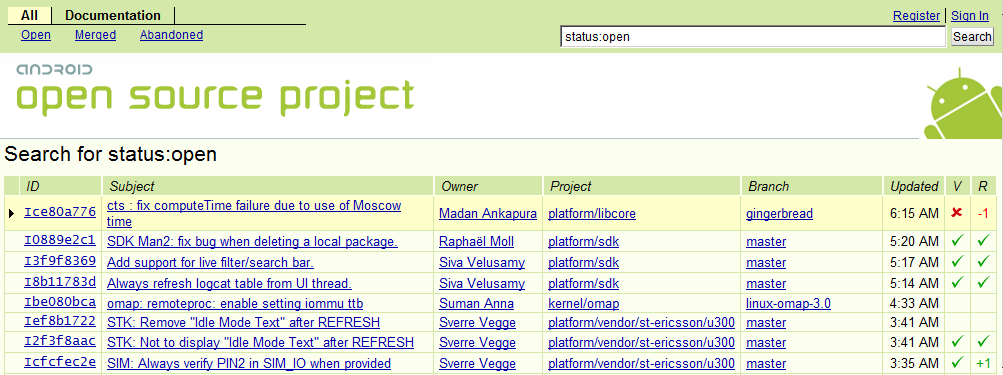
\includegraphics[keepaspectratio,width=\textwidth,height=0.75\textheight]{img/18333fig0202-tn.png}
\caption{Gerrit代码审阅系统}
\end{figure}

Gerrit是一个基于 Web 的代码评审和项目管理的工具,面向基于Git 版本控制系统的项目,所以如果你没用Git,就没法用Gerrit了,接下来看看在Gerrit中是怎么实施代码评审的。

\begin{itemize}
\item 首先开发者(贡献者)的代码变更通过Git命令被推送到Gerrit管理下的Git 版本库,推送的提交转化为一个一个的代码审核任务

\item 代码审核者可以通过Web界面查看审核任务、代码变更,通过 Web 界面做出通过代码审核(Review)或者拒绝(Reject)等决定。

\item 测试者(一般可以设定为持续集成的服务器执行)可以通过访问来获取代码变更进行相应测试,如果测试通过,就可以把这个评审任务设置为校验通过(Verified)。

\item 最后经过了审核和校验的代码变更可以通过Gerrit界面中提交动作合并到版本库的对应分支。

\end{itemize}

相比代码走读,它的好处在于,审阅动作发生在向主干提交代码前,可以只看变更的部分显得很贴心,网上随时随地审阅起来也很方便,这也是有别于结对编程的一个好处。

任何人都可以审阅提交的代码,整个团队的代码都一目了然,审阅起来更方便,非常符合开放、透明的敏捷精神。使用之后能够显著提高代码质量,甚至于等到习惯了以后,代码不被审阅一下,都觉得实在是不好意思提交到主干上去。

Gerrit中通过特定分支,任何审核任务的代码变更都能访问,所以如果需要细看或是合并到本地都异常的方便。

\section{Git的缺点}
\label{git的缺点}

相比SVN、Mercurial,Git的学习还是需要花更多的时间,但是掌握基本的命令就可以畅通无阻了。

如果你喜欢上了她,你可能会喜欢她的一切,对Git也如此。作为技术人员,看到一些小命令、小技巧,会越来越有兴趣。

所以努力克服一点小问题,越过这个门槛,前途会更加美好,就是我的建议。

\section{相关知识}
\label{相关知识}

GitHub、BitBucket、GoogleCode是非常流行的开源项目托管网站,也都支持Git,建议熟悉一下。

Mercurial(Hg)也是一个和Git相类似的分布式版本控制系统,可以了解一下。

\subsection{几种协议}
\label{几种协议}

访问远端仓库,大部分情况下使用SSH协议,实际上Git也可以用其他协议如\texttt{git:/\slash }和\texttt{http:/\slash },这些都是由Git服务器提供的服务。

\begin{lstlisting}[language=bash]
$ git clone ssh://git@gitserver/repo.git # 用git用户访问,常见于gitolite
$ git clone git@gitserver/repo.git  # SSH协议,和上面一样,ssh://省略了
$ git clone git@github.com:larrycai/sdcamp.git # SSH协议,用git用户访问,转到larrycai用户,常见于github
$ git clone larrycai@gitserver/repo.git # SSH协议,直接larrycai用户
$ git clone ssh://larrycai@gitserver:29418/repo.git # SSH协议,一般是Gerrit服务器
$ git clone git://gitserver/repo.git  # Git协议,一般用于克隆只读
$ git clone https://larrycai@gitserver/repo.git # HTTP协议,大部分情况是为了绕过防火墙
\end{lstlisting}

\section{课后练习}
\label{课后练习}

\begin{itemize}
\item 习惯使用Windows版的Git Bash环境。

\item 继续练习常用的例子:如熟练应用本地分支来开发任务、服务器同步。

\item 尝试用Gerrit给你所在产品的代码进行审阅。

\item 注册Github,并尝试提交本书的补丁。

\end{itemize}

\section{小结}
\label{小结}

Git是一个分布式版本控制系统,不应该用以前集中式的版本控制系统的思路去考虑。要反复练习来熟悉一些基本的用法,慢慢提高使用水平。

随着Git的日益普及,网上的资料已经很多,多问多玩。

Gerrit的代码审阅特别适合提高企业产品的代码质量,而且又不花费很多额外的时间。

\section{参考阅读}
\label{参考阅读}

\begin{enumerate}
\item Git权威指南:\href{http://www.worldhello.net/gotgit/}{http:/\slash www.worldhello.net\slash gotgit\slash }

\item Pro Git中文: \href{http://progit.org/book/zh/}{http:/\slash progit.org\slash book\slash zh\slash }

\item Git Community Book 中文版 \href{http://gitbook.liuhui998.com/}{http:/\slash gitbook.liuhui998.com\slash }

\item Gerrit \href{http://code.google.com/p/gerrit/}{http:/\slash code.google.com\slash p\slash gerrit\slash }

\item Windows版的Git:\href{http://code.google.com/p/msysgit/}{http:/\slash code.google.com\slash p\slash msysgit\slash }

\end{enumerate}

\chapter{持续集成}
\label{持续集成}

持续集成是一种软件开发实践,它是Martin Fowler先生提出\footnote{\href{http://martinfowler.com/articles/continuousIntegration.html}{http:/\slash martinfowler.com\slash articles\slash continuousIntegration.html}}的。它是一个在企业开发中必须的最基本的软件实践,谁也不会容忍企业的软件发布是在一台私人机器上完成的。

在持续集成中,团队成员频繁集成他们的工作成果,一般每人每天至少集成一次,在保证质量的同时也可以多次。每次集成会经过自动构建(包括自动测试)的验证,以尽快发现集成错误。许多团队发现这种方法可以显著减少集成引起的问题,并可以加快团队合作软件开发\footnote{\href{http://www.infoq.com/cn/articles/ci-theory-practice}{http:/\slash www.infoq.com\slash cn\slash articles\slash ci-theory-practice}}的速度。

在这一章中,我们先以一个简单的持续集成练习来体会一下,然后再来讨论企业中的持续集成和新动向。

\section{环境准备}
\label{环境准备}

服务器端准备好 Game of life项目的git仓库,客户端需要:

\begin{itemize}
\item Maven 2.x 包 \href{http://maven.apache.org/download.html}{http:/\slash maven.apache.org\slash download.html}

\item JDK 6 \href{http://www.oracle.com/technetwork/java/javase/downloads/index.html}{http:/\slash www.oracle.com\slash technetwork\slash java\slash javase\slash downloads\slash index.html}

\item Jenkins \href{http://jenkins-ci.org/}{http:/\slash jenkins-ci.org\slash }

\end{itemize}

\section{持续集成流程}
\label{持续集成流程}

持续集成的一个通常的简单流程如下:

\begin{enumerate}
\item 将已集成的源代码复制一份到本地计算机。(\texttt{git clone\slash pull})

\item 修改产品代码和添加修改自动化测试。

\item 把修改提交到源码仓库。(\texttt{git commit\slash git push})

\item 在持续集成服务器上基于主干(\texttt{master})的代码再做一次构建(编译,单元测试,构建,打包)。

\item 在持续集成服务器进行测试(验收)

\end{enumerate}

如果上述所有操作没有任何错误,没有人工干预,并通过了所有测试,我们才可以认为这是一次成功的构建。

\begin{figure}[htbp]
\centering
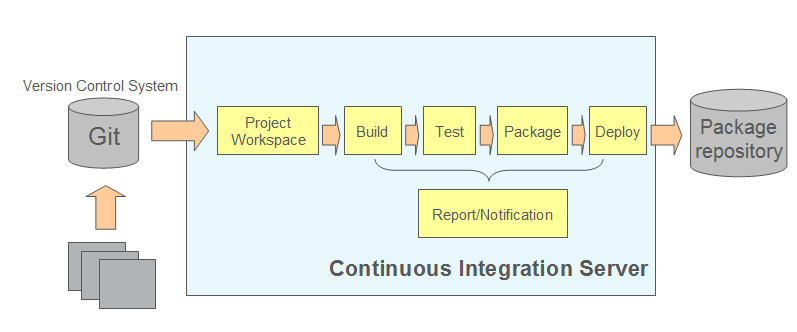
\includegraphics[keepaspectratio,width=\textwidth,height=0.75\textheight]{img/18333fig0301-tn.png}
\caption{持续集成流程}
\end{figure}

\section{Maven}
\label{maven}

Maven是一个Java项目管理工具,就像Make对于c\slash c++项目。在Java的构建中和它“类似”的是Ant和Buildr。Maven比Ant的好处\footnote{所有的好处坏处都因人而异,请不要计较。}是:

\begin{itemize}
\item 依赖包的管理只要写配置文件(\texttt{pom.xml})就可以了,而Ant需要把第三方依赖的二进制包放在项目里。

\item 定义了标准集合,简单了项目的管理。

\end{itemize}

Maven主要还包括:

\begin{itemize}
\item 一个项目对象模型 (Project Object Model)

\item 一组标准集合

\item 一个项目生命周期(Project Lifecycle)

\item 一个依赖管理系统(Dependency Management System)

\item 用来运行定义在生命周期阶段(phase)中插件(plugin)目标(goal)的逻辑。

\end{itemize}

\subsection{安装Maven}
\label{安装maven}

装好JDK6,熟悉Unix环境,用Git bash安装Maven

\begin{verbatim}
$ cd /c  # Windows C:/
$ tar -zxvf ~/Desktop/apache-maven-2.2.1-bin.tar.gz
$ mv apache-maven-2.2.1 maven
\end{verbatim}

在系统中配好环境变量\texttt{M2}、\texttt{M2\_HOME}、\texttt{MAVEN\_OPTS}、\texttt{PATH},如图3--2:

\begin{figure}[htbp]
\centering
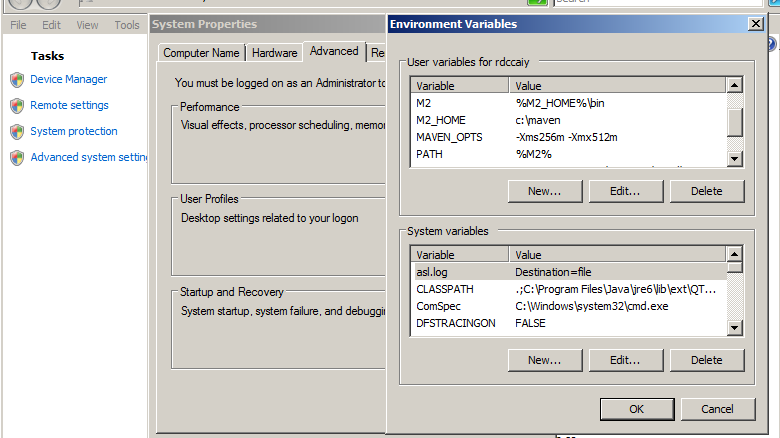
\includegraphics[keepaspectratio,width=\textwidth,height=0.75\textheight]{img/18333fig0302-tn.png}
\caption{系统中配好maven}
\end{figure}

别忘了,需要重新打开bash后,配置才会起作用。

\begin{verbatim}
$ mvn --version
Apache Maven 2.2.1 (r801777; 2009-08-07 03:16:01+0800)
\end{verbatim}

\subsection{Maven仓库管理器:Nexus}
\label{maven仓库管理器:nexus}

不管怎么样,Java的包在编译时还是要下载下来的,在企业中,最方便的是架设一个管理Java的包的服务器。其中最著名的就是Nexus,它会缓存远程仓库的Jar包。如图3--3 (源: http:/\slash today.java.net\slash article\slash 2010\slash 01\slash 04\slash maven-repository-managers-enterprise)

\begin{figure}[htbp]
\centering
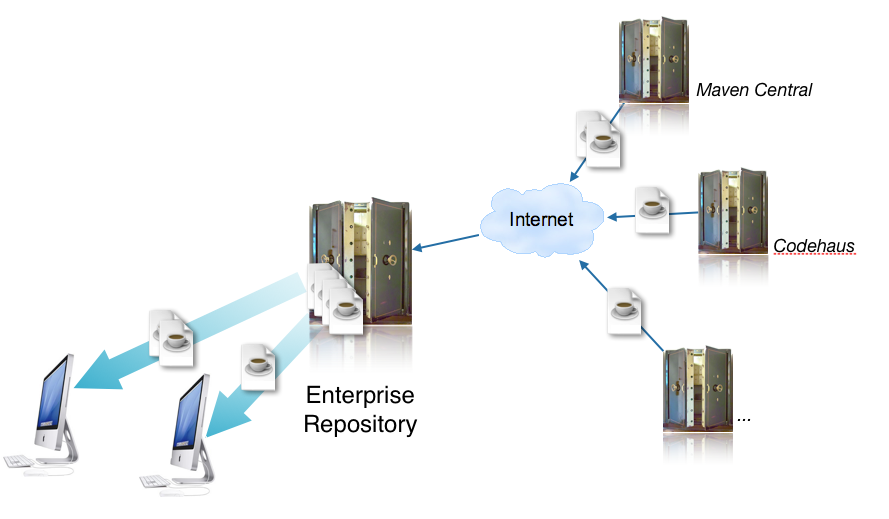
\includegraphics[keepaspectratio,width=\textwidth,height=0.75\textheight]{img/18333fig0303-tn.png}
\caption{Maven仓库管理器}
\end{figure}

对于个人来说,你不需要安装,只要在\texttt{\ensuremath{\sim}\slash .m2\slash settings.xml}配置指向企业使用的Nexus服务器就好了,如

\begin{lstlisting}[language=xml]
# ~/.m2/settings.xml
<settings>
 <mirrors>
  <mirror>
    <id>nexus</id>
    <mirrorOf>*</mirrorOf>
    <url>http://localhost:8081/nexus/content/groups/public</url>
  </mirror>
 </mirrors>
</settings>
\end{lstlisting}

\subsection{第一个maven命令}
\label{第一个maven命令}

在你的Game of life项目中,输入命令\texttt{mvn package},观察命令行的输出,并且查看 \texttt{\ensuremath{\sim}\slash .m2\slash repository}目录的变化。

第一次执行还是比较慢的,大量的Jar包会下载到本地的缓存中,稍后会看见需要的依赖都在\texttt{\ensuremath{\sim}\slash .m2\slash repository}中了。

\subsection{体会两层缓存}
\label{体会两层缓存}

实际上很容易理解,在个人机器上会有一个缓存,它在 \texttt{\ensuremath{\sim}\slash .m2\slash repository},在Nexus服务器上是整个公司项目的缓存。

在你第二次编译时速度明显快了。

\section{持续集成服务器:Jenkins}
\label{持续集成服务器:jenkins}

Jenkins是现在最流行也最有效的持续集成服务器,它的前身是著名的Hudson,后来由于Sun被Oracle收购以后,社区起了个新名字。

\subsection{安装}
\label{安装}

不需要安装,直接在命令行启动。

\begin{verbatim}
$ java -jar ~/Desktop/jenkins.war --httpPort=7080
\end{verbatim}

启动后就可以在你的浏览器中打开。\href{http://localhost:7080}{http:/\slash localhost:7080},用7080端口只是为了防止可能的8080端口冲突。

\subsection{安装Git插件}
\label{安装git插件}

Jenkins的强大得益于它的插件系统(以\texttt{.hpi}结尾),大部分情况下,你要的插件早在社区存在了。

为了使用Jenkins和Git服务器相连,你要安装Git插件。你可以选择从Jenkins系统中下载Git插件(如果公司有防火墙的话需要配Proxy),也可以直接把它下载到本地后,拷到\texttt{\ensuremath{\sim}\slash .jenkins\slash plugins}下,别忘了重启Jenkins服务器。这样你就能看到Git选项了。

\subsection{系统配置Maven}
\label{系统配置maven}

在系统中配置好maven目录,别忘了把自动安装选项去掉。

\begin{figure}[htbp]
\centering
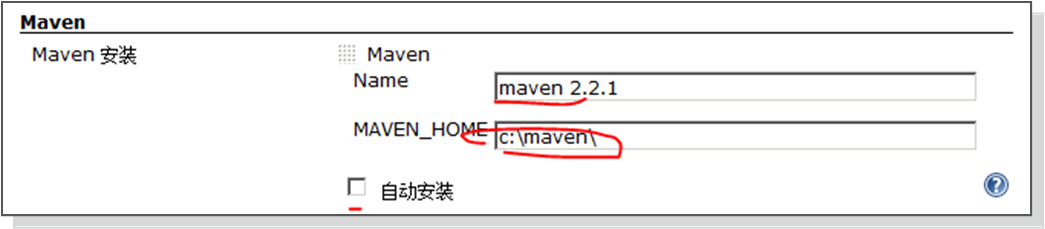
\includegraphics[keepaspectratio,width=\textwidth,height=0.75\textheight]{img/18333fig0304-tn.png}
\caption{Jenkins 系统配置Maven}
\end{figure}

\subsection{设置构建任务}
\label{设置构建任务}

新建一个任务\texttt{game-of-life},选择自由风格(freestyle)。

\begin{enumerate}
\item 源码管理:配置好Git的远端仓库。

\item 构建触发器:设置轮询(\texttt{Poll})策略:\texttt{*\slash 1 * * * *} (每分钟一次)

\item 构建:用\texttt{Invoke top-level maven targets}构建,填上\texttt{clean package}

\item 构建后操作: \texttt{Archive the artifacts}选中后填上\texttt{**\slash target\slash *.jar,**\slash target\slash *.war}

\end{enumerate}

\begin{figure}[htbp]
\centering
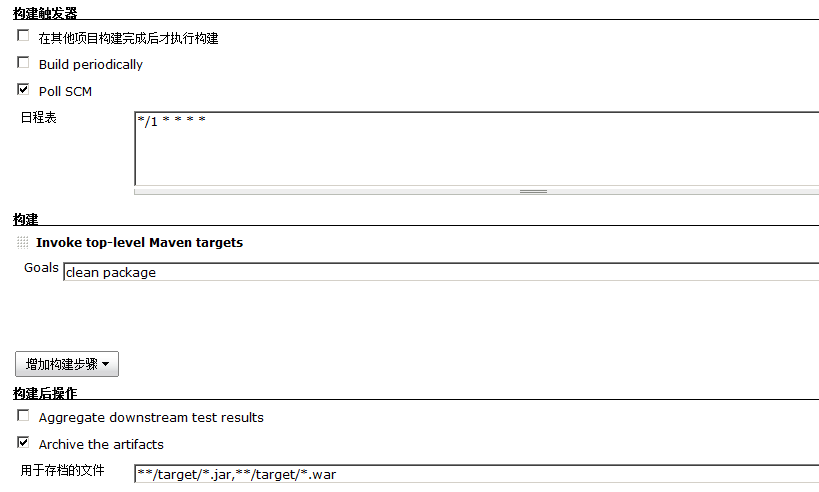
\includegraphics[keepaspectratio,width=\textwidth,height=0.75\textheight]{img/18333fig0305-tn.png}
\caption{Jenkins game-of-life配置}
\end{figure}

\section{企业中的持续集成}
\label{企业中的持续集成}

\section{如何实施持续集成}
\label{如何实施持续集成}

首要一步是把服务器架设起来,然后把你的脚本放在任务中自动执行。经常你会发现本地好好的,到了持续集成服务器就不对了。这是很常见的问题,基本上都是环境的影响。不管怎么样,要让团队明白,持续集成服务器构建出来的产品结果才是有效的。

其次持续集成是有团队负责的,要把结果透明化得显示在公共地方(如显示在电视上)。要养成集成失败后立马修复的好习惯,因为只要有一次没人修,慢慢的就没人用了。

\begin{figure}[htbp]
\centering
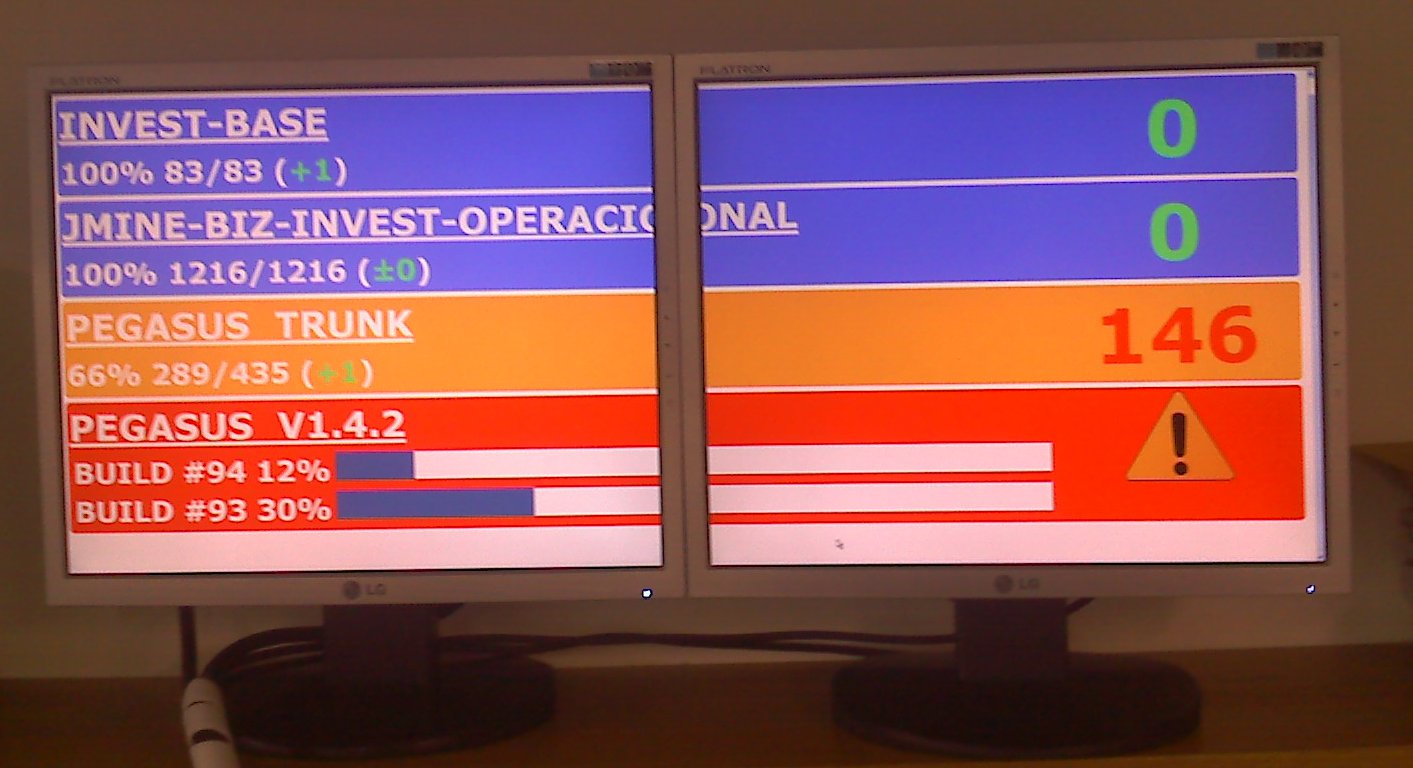
\includegraphics[keepaspectratio,width=\textwidth,height=0.75\textheight]{img/18333fig0306-tn.png}
\caption{Jenkins监控显示屏}
\end{figure}

此图来自\href{https://wiki.jenkins-ci.org/display/JENKINS/eXtreme+Feedback+Panel+Plugin}{Extreme Feedback Panel插件}\footnote{\href{https://wiki.jenkins-ci.org/display/JENKINS/eXtreme+Feedback+Panel+Plugin}{https:/\slash wiki.jenkins-ci.org\slash display\slash JENKINS\slash eXtreme+Feedback+Panel+Plugin}})。

最后要养成持续提高的工作态度,随着越来越多的东西加入持续集成,速度会变慢、经常出错。要不断的找到薄弱环节(bottleneck),查找相关技术来不断提高。

\section{相关知识}
\label{相关知识}

持续集成是十年前提出的东西,现在还有更多的好实践,建议看看持续交付一书。不仅产品代码需要持续集成,测试代码、基础设施的环境管理也需要持续集成。

在更多的持续集成上,要更进一步,达到持续交付。这并不一定代表你的产品一定需要在线运行,这更是一种软件开发的能力;你要很容易的部署到你的目标环境中,而且快速重现需要的配置。

\section{课后练习}
\label{课后练习}

\begin{enumerate}
\item 装一些插件(Raditor,cobertura)体会一下。

\item 把JUnit的单元测试结果显示出来。

\item 查找构建输出在哪里。

\item 和其他团队成员一起修改代码,并提交到代码库中,看看变化。

\end{enumerate}

\section{小结}
\label{小结}

持续集成是敏捷软件开发的重中之重,一定要养成好的习惯。

\section{参考阅读}
\label{参考阅读}

\begin{itemize}
\item Jenkins: The Definitive Guide:\href{http://www.wakaleo.com/books/jenkins-the-definitive-guide}{http:/\slash www.wakaleo.com\slash books\slash jenkins-the-definitive-guide}

\item Maven实战:\href{http://www.juvenxu.com/mvn-in-action/}{http:/\slash www.juvenxu.com\slash mvn-in-action\slash }

\item 持续集成软件质量改进和风险降低之道: \href{http://product.dangdang.com/product.aspx?product_id=20098017}{http:/\slash product.dangdang.com\slash product.aspx?product\_id=20098017}

\item 持续集成理论和实践的新进展: \href{http://www.infoq.com/cn/articles/ci-theory-practice}{http:/\slash www.infoq.com\slash cn\slash articles\slash ci-theory-practice}

\item Repository Management with Nexus : \href{http://www.sonatype.com/books/nexus-book/reference/index.html}{http:/\slash www.sonatype.com\slash books\slash nexus-book\slash reference\slash index.html}

\item 持续交付:\href{http://www.continuousdelivery.info/}{http:/\slash www.continuousdelivery.info\slash }

\end{itemize}

\chapter{如何写好Java程序}
\label{如何写好java程序}

写程序对每个软件开发者是个基本功,在企业中要考虑代码是给团队一起看的,因此质量的要求要更高一点。

首先你要有想把代码写好的意识,否者再怎么说都没用。可以经常想想你的代码几年以后还容易读吗?

如果你在用一些比较新的语言那就很幸运,因为有很多有效的工具支撑,Java程序看起来就比C\slash C++容易一点。

在个人环境下,如果用Eclipse,可以安装下面的很多插件来帮你自动做很多事情。主要考虑:

\begin{enumerate}
\item 代码覆盖率,对Java来说,90\%是一个不错的标杆,80\%很勉强。

\item 为了实现代码覆盖率,当然需要用到单元测试,JUnit 3\slash 4都可以,TestNG也不错。不用说,100\%通过是必须的。

\item 代码风格和一些常见错误会有 Checkstyle和FindBUGs\slash PMD\slash CPD等工具。

\end{enumerate}

怎么写好代码当然是更重要的事,你要熟悉基本的5大设计原则(SRP,OCP,LSP,DIP,ISP),理解这些以后,就可以学习如何用重构,如何用mock来隔离外部依赖写出好的单元测试。

测试驱动开发(TDD-Test Driven Development)是一个很有效的开发实践,要注重依据行为来驱动测试,而不是根据你的函数来写。

在服务器端,Sonar是个非常好用的工具,它把需要的质量信息都归纳起来了。一个产品架设好以后,代码的质量就一目了然了。

\begin{figure}[htbp]
\centering
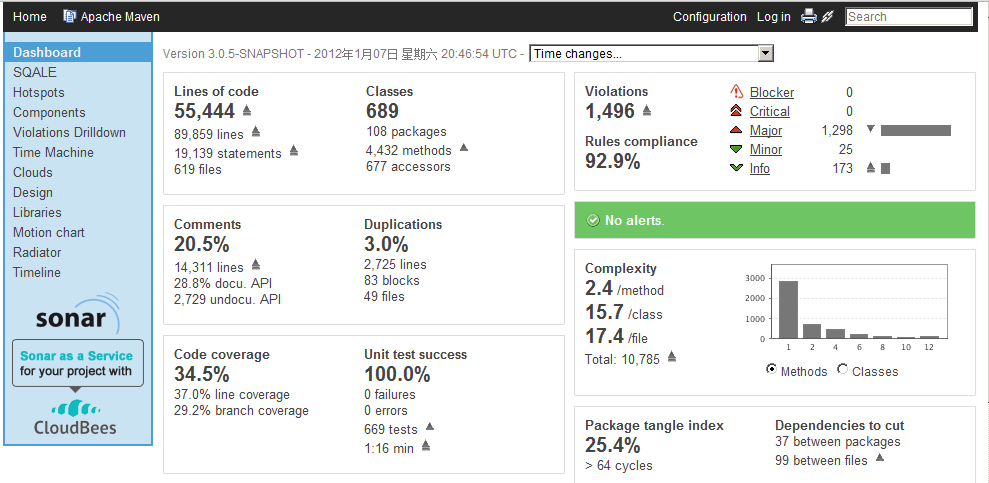
\includegraphics[keepaspectratio,width=\textwidth,height=0.75\textheight]{img/18333fig0401-tn.png}
\caption{Sonar}
\end{figure}

\section{环境准备}
\label{环境准备}

\begin{itemize}
\item Eclipse IDE和相关的插件EcmEmma

\end{itemize}

\section{代码风格和编程规范}
\label{代码风格和编程规范}

编程规范(代码风格)不需要自己去创立,继承别人现有代码就可以了,建议用\texttt{checkstyle}工具强制控制一些基本的。

下面列出一些常见的,不过重要的是理解,而不是事后检查。千万不要打印或制定厚厚的规范,没用的。可以翻翻\href{http://www.oracle.com/technetwork/java/codeconv-138413.html}{Java的编程规范}\footnote{\href{http://www.oracle.com/technetwork/java/codeconv-138413.html}{http:/\slash www.oracle.com\slash technetwork\slash java\slash codeconv-138413.html}},下面列出几个:

\begin{itemize}
\item 所有类的开头都要有Java文档的注释,而且写有用的内容。

\item 常量应该全部大写,单词之间由下划线分隔(例如,MAX\_WORK\_HOURS)。

\item 内部变量声明时应该对它进行初始化。

\item 不能有Magic数字,如\texttt{if(input\_length$<$8)}。

\end{itemize}

\section{安全代码}
\label{安全代码}

有些时候还要考虑一下写出安全的代码,这和产品的性质有关,web类产品会考虑得多一点。可以翻翻\href{http://www.oracle.com/technetwork/java/seccodeguide-139067.html}{Java的安全代码编程规范}\footnote{\href{http://www.oracle.com/technetwork/java/seccodeguide-139067.html}{http:/\slash www.oracle.com\slash technetwork\slash java\slash seccodeguide-139067.html}},下面列出几个:

\begin{itemize}
\item 要对输入信息(参数、特殊字符、SQL注入)进行检查验证。

\item 不要到处保存敏感数据(在数据库、文件等地方),如果必须要对它们进行保存,那就保存它们加密后的结果。

\item 要记录所有的或是有疑问的操作的日志。

\end{itemize}

\section{单元测试}
\label{单元测试}

这个应该是最简单的,但还是发现好多人都不做,要养成习惯,每个公共方法都需要至少有一个测试用例。

单元测试是代码的一部分,要养成同时签入版本库的习惯。而且如果本地没有100\%测试通过,也不允许提交代码。

良好的高度覆盖的单元测试是将来重构的保障。

\section{代码覆盖率}
\label{代码覆盖率}

有了单元测试后,就可以来看看代码覆盖率,建议在Eclipse中安装\href{http://www.eclemma.org/}{EclEmma}\footnote{\href{http://www.eclemma.org/}{http:/\slash www.eclemma.org\slash }},非常好用。

\begin{figure}[htbp]
\centering
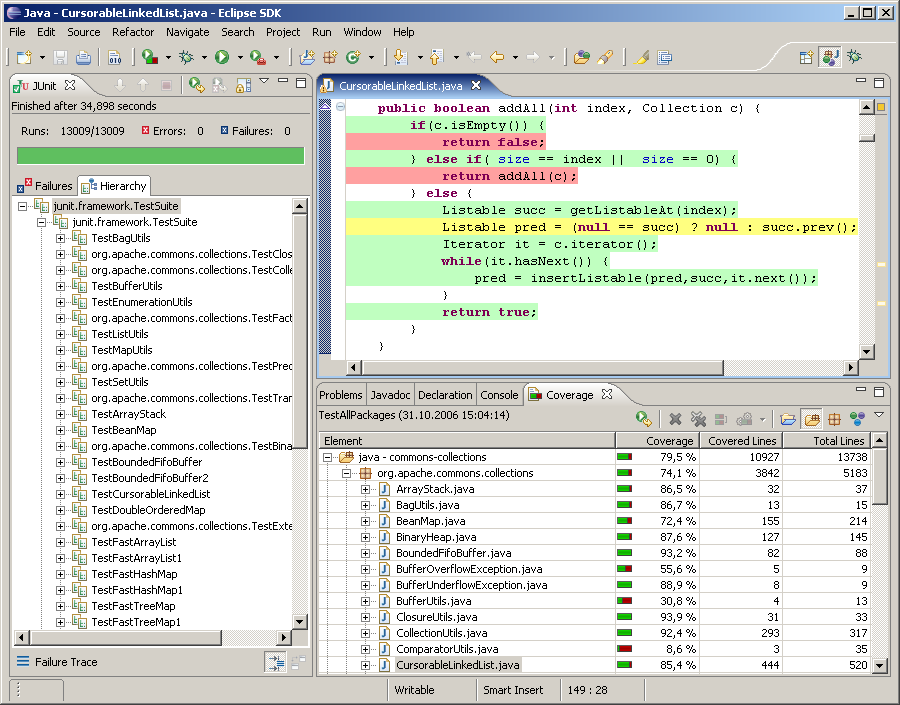
\includegraphics[keepaspectratio,width=\textwidth,height=0.75\textheight]{img/18333fig0402-tn.png}
\caption{Eclipse插件EclEmma}
\end{figure}

服务器端不用Sonar的话,cobertura不错。

\section{重构}
\label{重构}

重构分好几层,这里主要考虑日常的重构,千万不要跟经理或项目经理要求时间,这个是对他们不可见的,当然团队可以了解你重构的内容。

不要把重构当成很复杂的东西,大多数是很简单的,在Eclipse中点几下就可以了。

\begin{figure}[htbp]
\centering
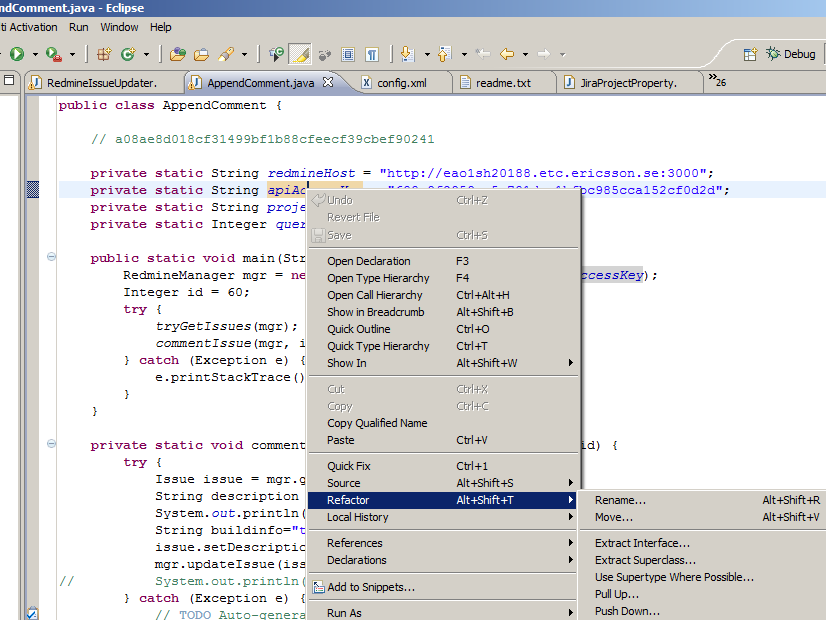
\includegraphics[keepaspectratio,width=\textwidth,height=0.75\textheight]{img/18333fig0403-tn.png}
\caption{Eclipse中使用Refactor}
\end{figure}

最常见的重构有:

\begin{itemize}
\item Rename (改名字)

\item Extract Method (提取函数)

\item Extract Interface (提取接口)

\end{itemize}

关键的是看到坏代码,要养成习惯去重构,基础是有质量高的单元测试。 

\section{测试驱动开发 TDD}
\label{测试驱动开发tdd}

很多人认为测试驱动开发会浪费时间,如果写完代码再写测试不更快捷吗?反正把覆盖率达到就好了。

代码覆盖率只是TDD的一个好处而已,以上正确的一个前提就是代码实现的是正确的需求,很多很多时候,我们写了很多的代码,但有部分是不必要的。代码的产量不重要,重要的是质量。过多的不必要的代码是浪费。

而且覆盖率补上往往是一种借口,大部分的人代码写完了,认为任务就完成了,单元测试是额外的工作,至少我看到蛮多项目经理就这么认为的。

测试驱动开发会把你写代码的速度慢下来,但确保你写出来的代码是有用的、干净的。

因此TDD会帮助我们让代码一直工作,并且保持干净。

\subsection{测试驱动开发的步骤}
\label{测试驱动开发的步骤}

典型的步骤是这样的:

\begin{enumerate}
\item 根据任务,新增一个单元测试用例(TestCase)。

\item 编译代码,让刚刚写的那个测试编译通过,运行会失败,在IDE中显示红条(Red Bar),因为还没有写实现代码。

\item 实现(implement)为了这个测试用例通过的代码,并编译通过。

\item 运行所有的测试,保证每个都能通过,在IDE中显示绿条(Green Bar)。

\item 重构代码,保持干净代码。

\end{enumerate}

\subsection{单元测试就是文档}
\label{单元测试就是文档}

如果你严格按照测试驱动开发方式来写代码,那么你的单元测试就应该是文档。

单元测试用例是为了实现某个功能而写的测试用例,因此它表明了代码的需求,读懂了这些需求,那就是很好的文档。

\subsection{单元测试也要重构}
\label{单元测试也要重构}

很多人只知道对实现代码进行重构,忘了单元测试也是很需要的。

所以建议你看看你的单元测试,是不是明白你的代码的作用了呢,如果不是,请重构。

\section{测试模拟(Mock)}
\label{测试模拟(mock)}

既然叫单元测试,那么它的目标一般就是一个方法,因此需要尽量小步、细粒度的来进行测试。这样单元测试才可以快速完成。

在现实情况下,很多方法往往依赖于其他一些难以操控的东西,这时就需要进行隔离,如网路、数据库连接等,这就需要使用Mock模拟。

同时Mock也保证了代码的可测性。

Mock一般都是通过接口(interface)来实现的,有很多Java工具来帮你Mock。老字号的有JMock、EasyMock,现在比较不错的工具\footnote{Stackoverflow 上的对这些工具的比较 \href{http://stackoverflow.com/questions/4105592/comparison-between-mockito-vs-jmockit-why-is-mockito-voted-better-than-jmockit}{http:/\slash stackoverflow.com\slash questions\slash 4105592\slash comparison-between-mockito-vs-jmockit-why-is-mockito-voted-better-than-jmockit}}是Mockito、JMockit、PowerMock。后面解决了一些EasyMock不能对复杂方法处理的弱点,特别是静态函数。

记住工具不是主要的,但是好的工具确实是很重要的。

\section{课后练习}
\label{课后练习}

\begin{enumerate}
\item 学习体会5大设计原则

\item 翻看代码规范,记住一些自己遗漏的地方。

\item 用TDD的方式实现一些功能,不要忘了重构和检查覆盖率。

\item 用JMockit工具来mock。

\end{enumerate}

\section{参考阅读}
\label{参考阅读}

\begin{enumerate}
\item The Principles of OOD : \href{http://butunclebob.com/ArticleS.UncleBob.PrinciplesOfOod}{http:/\slash butunclebob.com\slash ArticleS.UncleBob.PrinciplesOfOod}

\item 重构:\href{http://book.douban.com/subject/4262627/}{http:/\slash book.douban.com\slash subject\slash 4262627\slash }

\item 测试驱动的面向对象软件开发:\href{http://book.douban.com/subject/4910582/}{http:/\slash book.douban.com\slash subject\slash 4910582\slash }

\item EclEmma: \href{http://www.eclemma.org/}{http:/\slash www.eclemma.org\slash }

\item 测试驱动开发全功略@爬树的泡泡: \href{http://www.blogjava.net/briansun/archive/2005/07/31/8813.html}{http:/\slash www.blogjava.net\slash briansun\slash archive\slash 2005\slash 07\slash 31\slash 8813.html}

\end{enumerate}

\chapter{需求管理和实例化需求}
\label{需求管理和实例化需求}

在一个产品开发中,需求是推动整个软件开发的源泉。产品经理制定需求,确定了方向,但是如果方向(需求)一开始就有问题,后面开发测试得再辛苦、再认真、再正确,对产品来说都是不合格的。

现在代码质量的检测(如覆盖率,静态代码检测等等),持续集成技术都已经积累了很多的经验,能很好得保证编码阶段代码本身的质量。需求的BUG比开发中的BUG更难发现。那有没有有效的类似的工程实践来解决需求的问题呢?

在本章,我们一起来学习需求管理中现在来看蛮有效果的一种实践--\textbf{实例化需求(Specification by example)}。在下章同时会通过学习相关联的Cucumber软件来切身体会怎么将需求贯穿下去。

如果实施得好,相信你的产品的总体质量会上一个台阶。

\section{环境准备}
\label{环境准备}

纸和笔就可以了。

\section{需求的困惑}
\label{需求的困惑}

如果你做过开发,就知道软件开发的最大问题之一就是需求,而且它也很容易的被作为替罪羊。在公司项目延迟和出大问题的最大借口(不过这也是事实),就是“需求不清楚”。

那把需求早点弄清楚不就行了嘛?听着挺容易,但要做好它却很困难。

需求不清楚,不能开始项目,这一点大家都有共识。一种常见的解决办法就是:高级人员要对需求文档进行审核,完全通过后才能进行项目开发。但这实际上就是瀑布模型中的思路,大家已经知道它不大行得通,时间拉长了不算,早期把所有的需求都弄清楚也会变得纸上谈兵。

那敏捷迭代起来以后是否就好点呢。理论上会好点,因为需求在一个迭代中东西会少点,有机会理清楚一点。但就是因为一个迭代的周期短,在开完计划会议后(Planning meeting),团队会更愿意直接投入到代码开发中去,他们认为需求已经可以了;项目经理也觉得讨论需求会浪费点时间,我见过得很多人包括开发者都认为写代码才是干活。

这样的话,实际上往往到一个迭代的后面几天开始测试的时候才发现:测试人员、开发人员、产品负责人想的都不是很一样,但时间不够了,要不注册BUG,要不就是挪到下个迭代。这就是\textbf{技术债务(Technical Debt)}的最大根源。

那是否有好的办法把需求质量有效得提高?

\subsection{测试人员的工作文档}
\label{测试人员的工作文档}

测试人员应该除了产品负责人对需求是最了解得,至少比开发者知道得更多\footnote{很可惜这一点很多测试人员都没有体会到,他们很多时候都是被动得测。开发者做出什么,他们测什么。}。

再来看看现在的测试人员做了哪些事情,不同的公司可能不太一样,这里只是一种典型例子。

\begin{figure}[htbp]
\centering
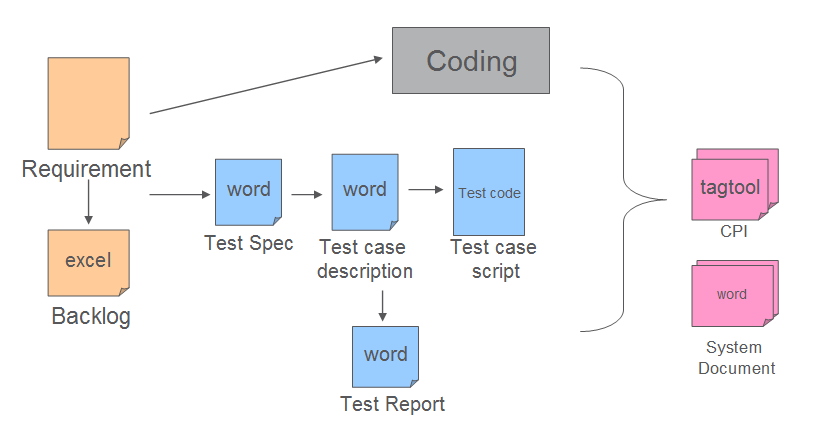
\includegraphics[keepaspectratio,width=\textwidth,height=0.75\textheight]{img/18333fig0501-tn.png}
\caption{测试人员的工作文档}
\end{figure}

得到“需求”后,首先可能要写的是\textbf{测试分析}:考虑一下这些功能大概的测试内容和范围。它存在的主要目的是为了让其他高级测试人员来把关,确保需求理解和相应的测试没有大的偏差,其中包括时间的估计。

紧接着是\textbf{测试用例}的描述:比较详细得用步骤的方式来阐述每一步测试。它很有可能是测试人员进行实际测试的主要文档,为了将来其他测试人员能重复测试。

如果运气好,敏捷实施不错的话,测试人员会被要求测试自动化,然后前一步骤的\textbf{测试用例}会被写成\textbf{测试脚本}。它来替换无谓的手工测试。再进一步,它还会在持续集成的服务器中被自动执行。

最后,一般都要求写一份\textbf{测试报告}:完成了多少测试用例等等。这个就是经理们经常想有的一份文档,以此来作为项目实施总结报告。

上面的每一步看上去都很有必要,缺一不可。

但我建议你在旁观者角度来精益软件角度观察一下,有没有浪费\footnote{精益软件开发的一大原则就是“消除浪费”,详见参考。}呢:

\begin{itemize}
\item 这些文档都有哪些人读呢?作用大吗?3年后还能读懂吗?

\item 可以合并一些文档吗?只有一份行不行呢?

\end{itemize}

\section{用实例化来解决需求的问题}
\label{用实例化来解决需求的问题}

解决需求当然有许许多多的办法,下面是几种常见的方式:

\begin{itemize}
\item 从TDD(测试驱动开发)引申出来的\textbf{ATDD(Acceptance Test Driven Development: 验收测试驱动开发)}。就是把TDD对开发者的成功经验挪到测试团队中,让测试人员在项目中起主导地位。

\item \textbf{BDD(Behavior Driven Development:行为驱动开发)}就是强调先搞清楚功能的业务需求,有它来指导后续的开发。

\item 实例化需求(Specification by Example):顾名思义就是要用例子的方式去阐述需求,这个概念是由\textbf{Gojko Adzic}提出的。

\end{itemize}

从本质上来说,实例化需求和ATDD、BDD包括其他的敏捷测试都是一个范畴,一样东西。但是实例化需求提出了更好得实践方式,减少了对工具的依赖,更容易被企业开发接受。

本章主要就是简单介绍实例化需求和实施的方法。

\subsection{主要过程模式}
\label{主要过程模式}

在【实例化需求】一书\footnote{图灵出版社已经引进出版,详见参考。}中,Gojko提出了实例化需求的主要过程模式

\begin{figure}[htbp]
\centering
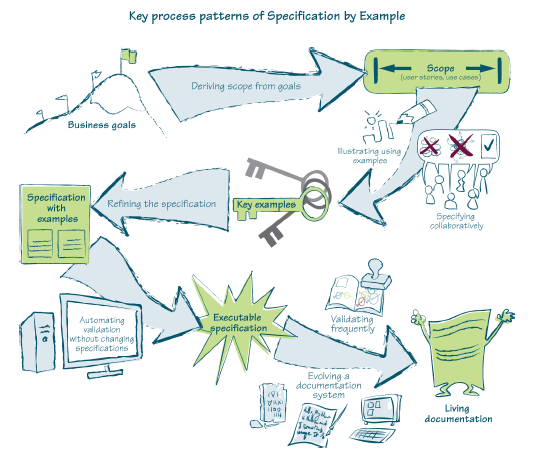
\includegraphics[keepaspectratio,width=\textwidth,height=0.75\textheight]{img/18333fig0502-tn.png}
\caption{实例化需求的主要过程模式}
\end{figure}

主要过程模式主要包括一下几个重要环节:

\begin{enumerate}
\item 从目标中获取范围:要一直牢记商业价值,为什么要做。很多时候执行项目时太关注怎么做了。

\item 用例子来协作探讨需求:例子能更好得把需求描述清楚,不能含糊。

\item 提炼需求说明:通过例子了解需求后就可以提炼出需要的需求说明。

\item 执行需求说明并自动化:需求说明如果能执行并放入到持续集成后,信息就不会过期。

\item 活文档:文档要长久,就必须要容易维护,从需求说明中自动产生出的活文档是最有效的方式。

\end{enumerate}

\subsection{网上书店一个例子}
\label{网上书店一个例子}

让我们先从一个常见的例子来学习一下,这个例子也是Gojko常用的,我可能在一些环节稍微改变了一下。

假设某个网上书店为了提高用户的回头率,就提出了口号:\textbf{到年末,达到50\%的用户的回头率},这就是\textbf{目标(Business Goal)}。一般是由CEO或最上层的市场经理根据市场决定的,他们关注的是战略方面的决策,也是整个产品开发的市场价值和背景。这一点经常被开发团队忽视,要让团队时刻知道项目的意义所在,这样在有冲突或对需求的理解产生怀疑时,就可以看看需求产生的具体原因,有时你可以想到不同的解决办法。条条道路通罗马-不过也要知道是去罗马对不对。

有了目标后,业务经理和领域专家们就可以从中提出一些要开发的项目\textbf{范围(Scope)},这个用头脑风暴(Brainstorming)的形式是最适当的,可能的产出点子如下:

\begin{itemize}
\item 给用户打折卡

\item 通过email主动推销优惠信息

\item 买书免运费

\item 限时打折

\item {\ldots} {\ldots}

\end{itemize}

这个阶段的关键是不要扼杀好点子,要集思广益。也不需要一开始就对点子进行细化,更多的是考虑投入产出比。在讨论充分的情况下,在会议的后期可以选定觉得最好的内容再进行推敲,以此来定出需求给研发部。

这一点就是关键,因为研发部一般和市场部不在一块儿(能在一块最好),通常是通过电子化的文档接受需求,这就一定要把需求说清楚,很显然用浅显易懂的语言来表示是最好的。先别看,你自己想想如果你来写会是什么样子。

好吧,让我们继续前面的例子。

假定\textbf{买书免运费}这个点子不错,现在就我们就可以试试用例子的方式来阐明需求。

\begin{itemize}
\item 一个普通客户买一本书,免运费。

\end{itemize}

听着不太划算,业务经理认为要有一定数量,那就先定6本吧,然后加上5本的测试例子使它更容易理解。

\begin{itemize}
\item 一个普通客户买6本书,免运费。

\item 一个普通客户买5本书,运费大于0。

\end{itemize}

蛮清楚的了,再来看看还有其他情况出现吗?

一个技术人员提出了运货范围,产品经理想了想竞争对手的情况,决定只给除西藏省,青海省的大陆地区免运费,差不多大家都清楚了。

\begin{itemize}
\item 一个普通客户买6本书,送货地址到上海,免运费。

\item 一个普通客户买6本书,送货地址到西藏,运费大于0

\item 一个普通客户买5本书,运费大于0。

\end{itemize}

还有吗?想了想,对了,买书的人经常顺便买个小电子产品(或化妆品,哈哈),让我们加个U盘的情况吧。

产品经理想想了,物流也不会有损失,同意。

\begin{itemize}
\item 一个普通客户买6本书,送货地址到上海,免运费。

\item 一个普通客户买6本书,送货地址到西藏,运费大于0

\item 一个普通客户买5本书,运费大于0。

\item 一个普通客户买6本书和一个U盘,送货地址到上海,免运费

\end{itemize}

反应快的立马想到了冰箱。

\begin{itemize}
\item 一个普通客户买6本书和一台冰箱,送货地址到上海,免运费???

\end{itemize}

要不要免呢?产品经理觉得自己做不了主,问物流经理。负责物流的业务经理连忙说吃不消了,因为大件电子商品的快递费用很高,要亏本的。行吧,那就不免吧。

\begin{itemize}
\item 一个普通客户买6本书和一台冰箱,送货地址到上海,运费大于0

\end{itemize}

这条和上面的U盘有冲突,需要解决。有人立马提出按重量来判断,大家一致同意。产品经理也定下了1公斤这个分界线。

\begin{itemize}
\item 一个普通客户买6本书,送货地址到上海,免运费。

\item 一个普通客户买6本书,送货地址到西藏,运费大于0

\item 一个普通客户买5本书,运费大于0。

\item 一个普通客户买6本书和一个小于1公斤的U盘,送货地址到上海,免运费

\item 一个普通客户买6本书和一台大于1公斤的冰箱,送货地址到上海,运费大于0

\end{itemize}

现在我们经过\textbf{集体下定义(Specifying Collaboratively)}得到了一下\textbf{关键例子(Key Examples)}。明显得,这种奇异是最少的,一目了然。主要原因是最自然的业务描述,人人都明白。

有了这些例子,又可以回头去审阅最原始的需求”买书免运费“,就可以\textbf{提炼需求说明(Refine the Specification)}来得到完整的\textbf{实例化的需求说明(Specification with examples)}。

\begin{verbatim}
需求:买书免运费
   提供读者买书优惠活动,买书超过(含)6本以上的而且重量小于1公斤,可以免费送货到除西藏省,青海省的大陆地区。
关键例子:
\end{verbatim}

\begin{itemize}
\item 一个普通客户买6本书,送货地址到上海,免运费。

\item 一个普通客户买6本书,送货地址到西藏,运费大于0

\item 一个普通客户买5本书,运费大于0。

\item 一个普通客户买6本书和一个小于1公斤的U盘,送货地址到上海,免运费

\item 一个普通客户买6本书和一台大于1公斤的冰箱,送货地址到上海,运费大于0

\end{itemize}

看上去很完美了,写入需求文档,放入Backlog,通知开发团队在下一个Spring中实现,争取早日上线。团队成员看了看,也觉得这次需求很清晰,也没问题,就承诺在这个Spring中完成。

孰料开发团队拿到这个需求准备实施没多久,架构师发现了个大问题:现在的数据库中没有“重量”一个字段,要加入这个字段的话,这个工作量会急剧上升。

怎么办呢?这是已经承诺好的需求,反悔还来得急吗?

软件开发中(生活中或亦如此)最重要的就是任何时候有问题,自己搞不定,不能完成自己的承诺时,都需要尽早提出来,和其他人一起商讨解决方案。

产品经理了解了技术难题后,认为这只是一个小的销售方案,没必要费那么多的开发时间。为了简化起见,大家一致决定只对图书免运费。

通过沟通,双方又都满意了。更新后的需求如下:

需求:买书免运费
 提供读者买书优惠活动,买书超过(含)6本以上而且只含书的订单,可以免费送货到除西藏省,青海省的大陆地区。
 关键例子:
 * 一个普通客户买6本书,送货地址到上海,免运费。
 * 一个普通客户买6本书,送货地址到西藏,运费大于0
 * 一个普通客户买5本书,运费大于0。
 * 一个普通客户买6本书和一个U盘,送货地址到上海,运费大于0

这些是最重要的步骤,如果能实践它,已经可以得益颇多了。关于怎么去执行,那得结合工具来讲,我会在下章解释。

\subsection{常见问题}
\label{常见问题}

在企业推动实例化需求,讲到这个例子时,经常会碰到这些问题:

\textbf{6件可配吗?}:例子中提到6件免运费,显然这个在系统中要可配的,不能在产品中硬编码(hard code)。但是这个需要在例子中讲清楚吗?

\begin{quote}

“否者我的开发团队又要说我需求没讲清楚,不过我总觉得这点意识他们应该有的?”,一个有着很多痛苦经历的PO问道。
\end{quote}

没有一定的说法。在这个案例中,建议没有必要把\textbf{免运费的数目可配}这个要求在例子中写出来。但是如果自己的团队这方面能力不够,提醒一下,或者放在基本要求中都是可以的。记住!!最重要的是沟通,把需求澄清出,不要有歧义。

\textbf{这不是Waterwall吗?}:这是一个简单的例子,看上去很快就弄明白了。但是在实际中,有太多的需求要澄清呀?

\begin{quote}

”这样看上去和以前没有两样,还是要花好多时间来搞清需求,只是快了一点而已?“
\end{quote}

不是的,在实际运作中,这是一个迭代式得不断澄清的过程,可以把最重要的先澄清。这里面还有一个很重要的是:就算在优先级最高的需求中也有不重要的小功能,这个用例子的方式很容易体现出来。

\textbf{和用例有区别吗?}:很多人初次接触这个时总觉得和用例没区别。

可能,但是我很少看到好的用例,用例很多时候关注在技术实现的步骤上了,所以有很多不必要的技术细节,不太适合产品经理来阅读。这儿我们要求的是一份大家都能容易读懂最少歧义的需求。

当然不排除你的用例很容易读,没有冗余,那往往就是实例化了。

\section{如何实施}
\label{如何实施}

以前在估计时间时,团队很容易用含糊的原因解释。敏捷实施中又要求团队来估时间,常见的毛病就是:

\begin{quote}

我们需要1000人时(manhour),300人时是准备环境,400设计加开发,300人时是测试。
\end{quote}

现在用实例化需求后,很容易得针对每个例子来估时间,PO也可以根据时间的代价来取舍。

认可了这种实践,实施起来也相对容易一点,下面列出几个要点(需要不断学习)。

\subsection{循序渐进和现有流程的结合}
\label{循序渐进和现有流程的结合}

我们可以不用改变现有流程的方式把实例化需求循序渐进的开展起来,这一点在企业中很重要,大的改变都很费周折。

在\textbf{测试分析}阶段,我们可以把简单的需求列出来,加上理解的一个最重要的例子就可以了。可以结合迭代式的方式,优先级高的先多花时间来写\textbf{测试用例}。

当然在写\textbf{测试用例}时,我们可以继续前面的格式,只是多加几个例子,并且持续地提炼需求说明,使得越来越清晰。

在下章中介绍如何把\textbf{测试用例}直接变成可测试的\textbf{测试脚本}。

这样子,你的现有流程就不需要改变,如果你已经有现成的框架来做\textbf{测试脚本},那就继续用下去吧,只要需求明白了,什么都好解决。

\subsection{贴在墙上}
\label{贴在墙上}

把需求贴在墙上可视化一点也是非常有效果的,它可以减少浪费。企业最大的毛病就是会多,每个人都是认为自己的会重要,这是很浪费时间的。

完全不一定每次审阅都要去参加,只要我们把需求贴在墙上,团队就随时随地得可以了解最新的进展。随手拿个即时贴提建议:时间估计,架构的影响{\ldots}

如果对某个需求需要讨论了,召集相关人(千万不要整个团队)在小房间搞清楚,然后立即更新需求。

因为我们现在用上了自然语言的实例化的需求,任何时候团队成员应该很容易读懂,而且没有偏差;如果有,说明还不清楚。

\section{相关知识}
\label{相关知识}

\begin{itemize}
\item 了解ATDD,BDD

\item 阅读从用户体验中挖掘需求一种方式``体验设计7日谈之一:关于软件的体验设计'':\href{http://www.infoq.com/cn/articles/xzc-experience-design-software}{http:/\slash www.infoq.com\slash cn\slash articles\slash xzc-experience-design-software}

\item 了解特性注入(Feature Injection): \href{http://www.infoq.com/cn/news/2009/05/feature-injection-comics}{http:/\slash www.infoq.com\slash cn\slash news\slash 2009\slash 05\slash feature-injection-comics}

\end{itemize}

\section{课后练习}
\label{课后练习}

\begin{itemize}
\item 试着把身边最近工作过的一个需求用这种方式体会一下。

\end{itemize}

\section{小结}
\label{小结}

实例化需求是一种很棒的协作探索需求的好办法,它强调了无时不刻地沟通的必要性,还有就是用例子来讲述需求更容易理解。但是要用熟练了还是很有难度得。

\section{参考阅读}
\label{参考阅读}

\begin{enumerate}
\item Book: Specification by example. \href{http://manning.com/adzic}{http:/\slash manning.com\slash adzic}

\item Specification by example: \href{http://specificationbyexample.com}{http:/\slash specificationbyexample.com}

\item 精益软件开发: \href{http://zh.wikipedia.org/zh/%E7%B2%BE%E7%9B%8A%E8%BD%AF%E4%BB%B6%E5%BC%80%E5%8F%91}{http:/\slash zh.wikipedia.org\slash zh\slash \%E7\%B2\%BE\%E7\%9B\%8A\%E8\%BD\%AF\%E4\%BB\%B6\%E5\%BC\%80\%E5\%8F\%91}

\item 实例化需求中文书:\href{http://www.ituring.com.cn/book/837}{http:/\slash www.ituring.com.cn\slash book\slash 837}

\end{enumerate}

\chapter{用Cucumber来实例化需求}
\label{用cucumber来实例化需求}

在上一章中我们已经了解如何把需求用实例化的方式弄清楚,现在继续考虑怎么用通用的记录下来,并且去执行它。

这方面实际上有很多工具,在本章,我们会通过学习一种现在最有效的Cucumber软件来切身体会怎么将需求贯穿下去,其他的可以看相关知识。

开始前,再强调一下,滥用工具还不如不用,Cucumber也是如此。

\section{环境准备}
\label{环境准备}

\begin{itemize}
\item Windows下的Ruby \href{http://rubyinstaller.org}{http:/\slash rubyinstaller.org}

\end{itemize}

\section{Cucumber 简介}
\label{cucumber简介}

Cucumber(英文:黄瓜)(官方网站是\href{http://cukes.info/}{http:/\slash cukes.info\slash })是一个实例化需求的极佳实现伴侣。它是基于Ruby的开源测试工具,得益于Ruby便于创建和使用DSL的特性,它可以通过自然语言(文本文字)来描述需求(业务层),并通过关键字驱动和正则表达式匹配告诉去做哪些事情(驱动层),在运行自动化测试结束以后,还会给出详细的报告。

\begin{figure}[htbp]
\centering
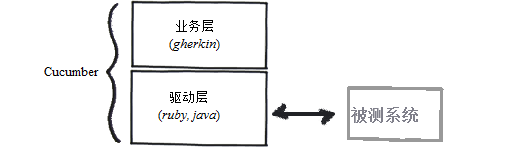
\includegraphics[keepaspectratio,width=\textwidth,height=0.75\textheight]{img/18333fig0601-tn.png}
\caption{Cucumber的架构}
\end{figure}

下面就是一个加法例子的需求描述,Cucumber文件以\texttt{.feature}结尾。

\begin{verbatim}
# 加法 adding.feature
Feature: Adding
  In order to avoid silly mistakes
  As a math idiot
  I want to be told the sum of two numbers
  
  Scenario: Add two numbers
    Given the input "2+2"
    When the calculator is run
    Then the output should be "4"

  Scenario Outline: Add two numbers
    Given the input "<input>"
    When the calculator is run
    Then the output should be "<output>"
    Examples:
      | input | output |
      | 2+2 | 4 |
      | 98+1 | 99 |
\end{verbatim}

这就是业务层,它和上一章最后的例子很像。功能标题后面是它的简要描述,然后是详细的例子。

建议好好读读Dan Nothy的文章:什么是故事\href{http://dannorth.net/whats-in-a-story/}{http:/\slash dannorth.net\slash whats-in-a-story\slash }。

现在让我们试着来运行它,看看会怎么样。

\section{安装}
\label{安装}

在Windows上,RubyInstaller提供了ruby的环境,下载安装包(如\texttt{rubyinstaller-1.9.3-p0.exe}),运行即可,别忘了把“Ruby放入PATH中”的选项选上。

\begin{figure}[htbp]
\centering
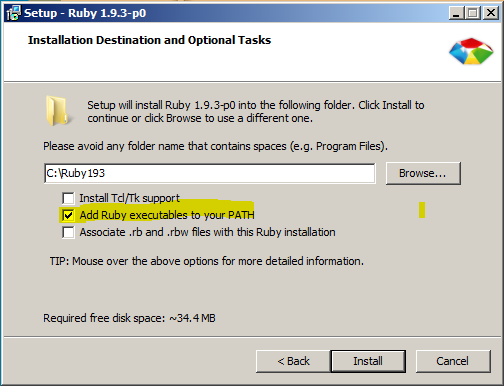
\includegraphics[keepaspectratio,width=\textwidth,height=0.75\textheight]{img/18333fig0602-tn.png}
\caption{Windows平台安装Cucumber}
\end{figure}

\$ gem install cucumber \# 如果需要配代理,-p http:/\slash :
 \$ gem install rspec \# cucumber 需要

\section{运行Cucumber}
\label{运行cucumber}

一旦Cucumber装好了,我们就可以使用 cucumber 命令来运行feature文件。

feature文件放在\texttt{features}目录下,如果cucumber命令后不跟任何东西的话,那么它会执行所有的.feature文件。如果我们只想运行某一个.feature文件,我们可以使用命令 \texttt{cucumber features\textbackslash{}feature\_name}

\$ cucumber features\slash adding.feature
 Feature: Adding
 In order to avoid silly mistakes
 As a math idiot
 I want to be told the sum of two numbers

\begin{verbatim}
Scenario: Add two numbers       # features\adding.feature:3
  Given the input "2+2"         # features\adding.feature:4
  When the calculator is run    # features\adding.feature:5
  Then the output should be "4" # features\adding.feature:6

Scenario Outline: Add two numbers      # features\adding.feature:8
  Given the input "<input>"            # features\adding.feature:9
  When the calculator is run           # features\adding.feature:10
  Then the output should be "<output>" # features\adding.feature:11

  Examples:
    | input | output |
    | 2+2   | 4      |
    | 98+1  | 99     |
\end{verbatim}

3 scenarios (3 undefined)
 9 steps (9 undefined)
 0m0.046s

You can implement step definitions for undefined steps with these snippets:

Given \slash \textsuperscript{the} input ``(\footnote{"}*)''\$\slash  do \textbar{}arg1\textbar{}
 pending \# express the regexp above with the code you wish you had
 end
 {\ldots}

你就可以看到它被正常执行了,发现了3个场景(scenarios),9个步骤(steps),这不就是我们需要的测试吗!!

让我们来解读一下吧。

\section{业务层:Gherkin语言}
\label{业务层:gherkin语言}

业务层实际使用的是\href{gherkin}{Gherkin语言}\footnote{\href{gherkin}{gherkin}},Cucumber是一个解释程序,它用来执行解释 .feature文件里业务描述,它的关键字就是“Given”、“And”等等这样的字眼。

一个常见的Cucumber文件描述分为 \textbf{Feature(特性)}、\textbf{Scenario(场景)}、和\textbf{Step(步骤)}。让我们再来看看上面的例子:

\begin{enumerate}
\item \texttt{Feature: Adding}: 这是标题,每一个feature文件以关键字\textbf{Feature}开始,且紧跟着一个冒号和一个简单描述。

\item 在上面,你发现接下来的几行描述不会被解析,纯粹是描述用的(当然也很重要),强烈建议你照\textbf{用户故事(User Story)}的方式去写。

\item \texttt{Scenario: Add two numbers}:关键字\_Scenario\_后面紧跟一个冒号和一个对应该场景的描述,也是简短的一句话。

\item 后面的以\textbf{Given\slash When\slash Then\slash And\slash But}开头(这些也是关键字)的都是步骤(步骤后面不需要跟冒号),用来阐述到底要的是什么样的需求。

\item \texttt{Scenario Outline: Add two numbers}: 关键字Scenario Outline,和Scenario不同的是它是支持表格的形式。

\item \textbf{Scenario} 和 \textbf{Scenario Outline}提供了特性的多个场景,可以出现多次。\textbf{Scenario Outline}提供了表格的形式,适合批量数据的处理。

\end{enumerate}

具体怎么连到被测系统就靠驱动层了。

\section{驱动层}
\label{驱动层}

驱动层的主要目的就是把业务层中的数据(如上“2+2”,“加”)提取出来,通过于应用程序进行交互,最后把返回结果和预期的值(“4”)进行比对,得出测试结果。

Cucumber的驱动层可以用Ruby,Java和其他语言来支持,很多时候语言的选择主要依赖团队的兴趣。这里以Ruby为例,当然不用担心,因为介绍的例子不需要很多深奥的知识。

在Cucumber中,第一次运行后,它会给出Ruby代码的模板,就是:

Given \slash \textsuperscript{the} input ``(\footnote{"}*)''\$\slash  do \textbar{}arg1\textbar{}
 pending \# express the regexp above with the code you wish you had
 end
 {\ldots}

如果对脚本或Linux比较了解的话,很容易看出,这是一个正则表达式。

在\texttt{features}下面建一个\texttt{step\_definitions}目录,把上面运行的代码模板片段写入\texttt{calculator\_steps.rb}文件中,并且把\texttt{pending}那一行用\texttt{\#}注释掉,再次运行\texttt{cucumber},就很顺利通过了。

3 scenarios (3 passed)
 9 steps (9 passed)

真实情况下,我们要写些代码匹配到关键字处理后,想办法传递到被测的系统,并和设定的期望值匹配来确定测试结果。

\section{常用的目录结构}
\label{常用的目录结构}

常用的目录结构组织方式是

\begin{lstlisting}[language=bash]
$ find calculator
calculator/
calculator/feature.html
calculator/features
calculator/features/adding.feature
calculator/features/division.feature
calculator/step_definitions
calculator/step_definitions/calculator_steps.rb
\end{lstlisting}

\begin{enumerate}
\item \texttt{features}下面按功能放置各个业务。

\item \texttt{step\_definitions}存放驱动层的脚本。

\end{enumerate}

\section{继续网上书店的例子}
\label{继续网上书店的例子}

Cucumber虽然上是支持多语言包括中文\footnote{61}的,但还是建议关键字用英文来写,以免其他工具的不支持。

用Cucumber重写的话,下面是一种方案。

\# book.feature
 Feature: 买书免运费
 提供读者(不管普通还是VIP客户)买书优惠活动,
 买书超过(含)6本以上的,可以免费送货到除西藏省,青海省的大陆地区。
 Scenario Outline:
 Given 一个客户买了 $<$几本书$>$
 And 买了 $<$其他类别$>$ 的东西
 When 选好 $<$送货地址$>$
 Then 看见 $<$运费为0$>$

\begin{verbatim}
  Examples:
  | 几本书| 其他类别 | 送货地址 | 运费为0 |
  |  6    | n/a      | 上海     |  yes    |
  |  6    | n/a      | 西藏     |  no     |
  |  5    | n/a      | 上海     |  no     |
  |  6    |          | 上海     |  no     |
\end{verbatim}

它对应的用Ruby实现的驱动层的代码就可以类似:

\begin{lstlisting}[language=ruby]
  def onlinebookstore(book_number,other_order_category,delivery_address)
    # 写代码发往被测系统,得到运费
      return 10 #模拟运费10元
  end
  Given /^一个客户买了 (\d+)$/ do |number|
    @book_number = number
  end
  Given /^买了(.*) 的东西$/ do |category|
    @order_category = category
  end
  When /^选好 (.*)$/ do |address|
    @delivery_address = address
    @result = onlinebookstore(@book_number, @order_category,@delivery_address)
  end
  Then /^看见 (yes|no)$/ do |expected_output|
    if(expected_output == 'yes')
      @result.should == 0
    else
      @result.should == 1
    end
  end    
\end{lstlisting}

所以运行后,你应该能够从输出结果中看到3个Scenario测试通过了。

4 scenarios (1 failed, 3 passed)
 16 steps (1 failed, 15 passed)
 0m0.076s

如果你上过TDD了,就知道现在我演示的只是模拟的实现,现在就是驱动你把驱动层的代码写好使他被运行通过。

怎么样,有点感觉了,多多练习吧。

\section{常见问题}
\label{常见问题}

\subsection{我们的系统没有接口能够被这么(或容易)测试得?}
\label{我们的系统没有接口能够被这么(或容易)测试得?}

好问题!!上面这个网上书店系统

\begin{itemize}
\item 可能使用Flash写的,你根本没法用脚本填充数据,然后得到结果。

\item 或者就算是用HTML5写的,但是调用它也是很费时间周折的呀。

\end{itemize}

是的,没错测试是费时的,但再想想背后的原因!

这就是没有测试驱动开发的后果,任何技术的设计不仅要考虑实现,也要考虑测试,\textbf{应用程序是否能够被自动化测试}是一个衡量软件开发水平的重要标志。否者要架构师干嘛?

\subsection{Cucumber用起来了,也自动化了,但是没人看?}
\label{cucumber用起来了,也自动化了,但是没人看?}

正常。不要为了Cucumber而Cucumber;不要为了自动化而自动化。

首先要理解实例化需求,然后再用工具去支持,不能本末倒置。

另外把结果变成网页或者贴在墙上都是不错的建议,试试下面的命令吧?

\$ cucumber --format progress --format html --out=features\_report.html

看看HTML的输出,你也可以自己定制你的报告。

\begin{figure}[htbp]
\centering
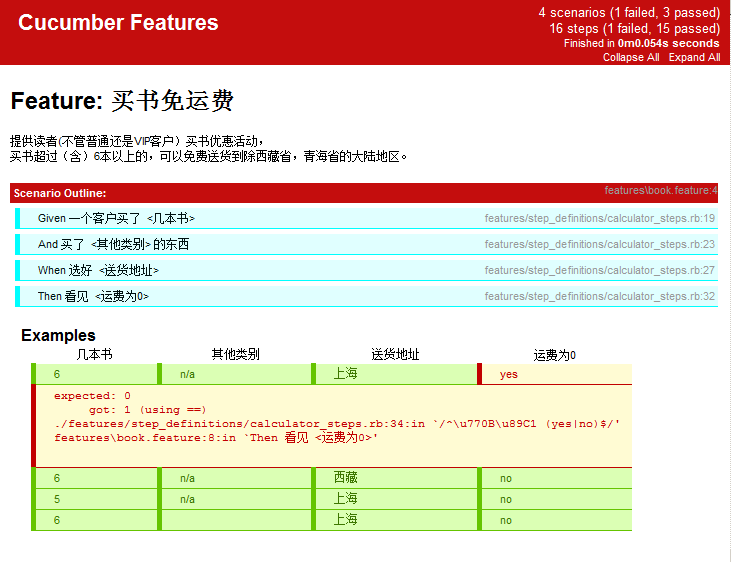
\includegraphics[keepaspectratio,width=\textwidth,height=0.75\textheight]{img/18333fig0603-tn.png}
\caption{Cucumber的架构}
\end{figure}

\section{相关知识}
\label{相关知识}

\begin{itemize}
\item \href{http://fitnesse.org/}{FitNesse}\footnote{\href{http://fitnesse.org/}{http:/\slash fitnesse.org\slash }}也是ATDD中很著名的一种工具,在Cucumber前占有很大的地位。

\item \href{http://blog.csdn.net/kerryzhu/article/details/6752992}{敏捷测试的思考和新发展}\footnote{\href{http://blog.csdn.net/kerryzhu/article/details/6752992}{http:/\slash blog.csdn.net\slash kerryzhu\slash article\slash details\slash 6752992}}

\end{itemize}

\section{课后练习}
\label{课后练习}

\begin{enumerate}
\item 把网上书店的例子,尝试用实例化需求说明的方式来描述清楚,并写成Cucumber的格式。

\item 阅读参考书,了解更多的Cucumber知识。

\item 了解Gherkin语言的详细内容,如\textbf{tag},并结合Cucumber去执行。

\item 看看如何能够实施Cucumber,使它能够整合到持续集成中去。

\end{enumerate}

\section{小结}
\label{小结}

Cucumber也只是一种工具,如果不理解实例化需求说明的真正意义,它会被用得很累,好自为之。

\section{参考阅读}
\label{参考阅读}

\begin{enumerate}
\item Book: Specification by example. \href{http://manning.com/adzic}{http:/\slash manning.com\slash adzic}

\item Specification by example \href{http://specificationbyexample.com}{http:/\slash specificationbyexample.com}

\item Cucumber \href{http://cukes.info}{http:/\slash cukes.info}

\item Gherkin语言:\href{https://github.com/cucumber/cucumber/wiki/Gherkin}{https:/\slash github.com\slash cucumber\slash cucumber\slash wiki\slash Gherkin}

\item Book: The Secret Ninja Cucumber Scrolls: \href{http://cuke4ninja.com/}{http:/\slash cuke4ninja.com\slash }

\end{enumerate}

\chapter{项目实践-Game of life}
\label{项目实践-gameoflife}

如果你是在自学,那么请用你自己的项目结合前面学到的东西练习一下,最好和几个同事一起来做。

如果你参加了公司的培训,这会是紧张和忙碌的一天。

作为团队,你们会收到产品负责人布置的任务,请用学到的东西去实践,记住团队合作!

练习的项目是取自John的\href{http://www.wakaleo.com/books/jenkins-the-definitive-guide}{Jenkins指南}\footnote{\href{http://www.wakaleo.com/books/jenkins-the-definitive-guide}{http:/\slash www.wakaleo.com\slash books\slash jenkins-the-definitive-guide}}中的演示代码-\href{https://github.com/wakaleo/game-of-life}{生命游戏(game of life)}\footnote{\href{https://github.com/wakaleo/game-of-life}{https:/\slash github.com\slash wakaleo\slash game-of-life}}

\section{常见问题}
\label{常见问题}

无论你多么强调团队合作的重要性,一碰到实际的项目,往往什么都忘了,下面是常见的两个毛病。

\subsection{过度承诺(over commit)}
\label{过度承诺(overcommit)}

大部分人觉得任务很简单,一会儿就做完了,可往往一天都没完成,完成的最差\footnote{不过这个团队可能收获也是最多的。}的是0。

而且一般都不会主动和产品负责人去沟通,提前汇报风险,使得产品负责人早作准备。都要在产品评审会议的时候才会说不行了,太晚了。

\subsection{没有团队精神}
\label{没有团队精神}

讨论任务的时候还有点点团队精神,但是领完任务后又立马单枪匹马的干活了,最多是两人一组。一般一个两人的小组忘了他们是一个大团队,没有想到要帮助别人,关心其他团队成员。

\subsection{缺少计划和工作方式的制定}
\label{缺少计划和工作方式的制定}

没有规矩,不成方圆。很多情况下,团队常常匆忙开始开发工作,而忽略了必要的团队计划和工作方式制订。主要原因是时间很紧,需求很多,环境不熟悉。大家在如此巨大的压力下,往往会选择马上开始动手,而忘记了‘磨刀不误砍柴功’的古训。

这样的后果是, 一旦有任何意外发生,团队会陷入混乱状态,完全没有办法给出相应的应对措施。同时,由于缺少统筹安排,团队分工不明,会导致不必要的浪费。

\section{小结}
\label{小结}

怎么样,经过一天的实战,体会到了企业开发的皮毛了吗?这还刚刚开始,享受你的企业敏捷开发之旅吧。
